\begin{enumerate}[label=\thesubsection.\arabic*.,ref=\thesubsection.\theenumi]
\numberwithin{equation}{enumi}
\item
Sketch the Polar Plot of
\begin{align}
G\brak{s} = \frac{\brak{1+\frac{s}{29}}\brak{1+0.0025s}}{\brak{s^{3}}\brak{1+0.005s}\brak{1+0.001s}}
\end{align}

\solution 
%
The following code generates the polar plot in Fig.   \ref{fig:ee18btech11029}

\begin{lstlisting}
codes/ee18btech11029.py
\end{lstlisting}

\begin{figure}[!h]
\centering
  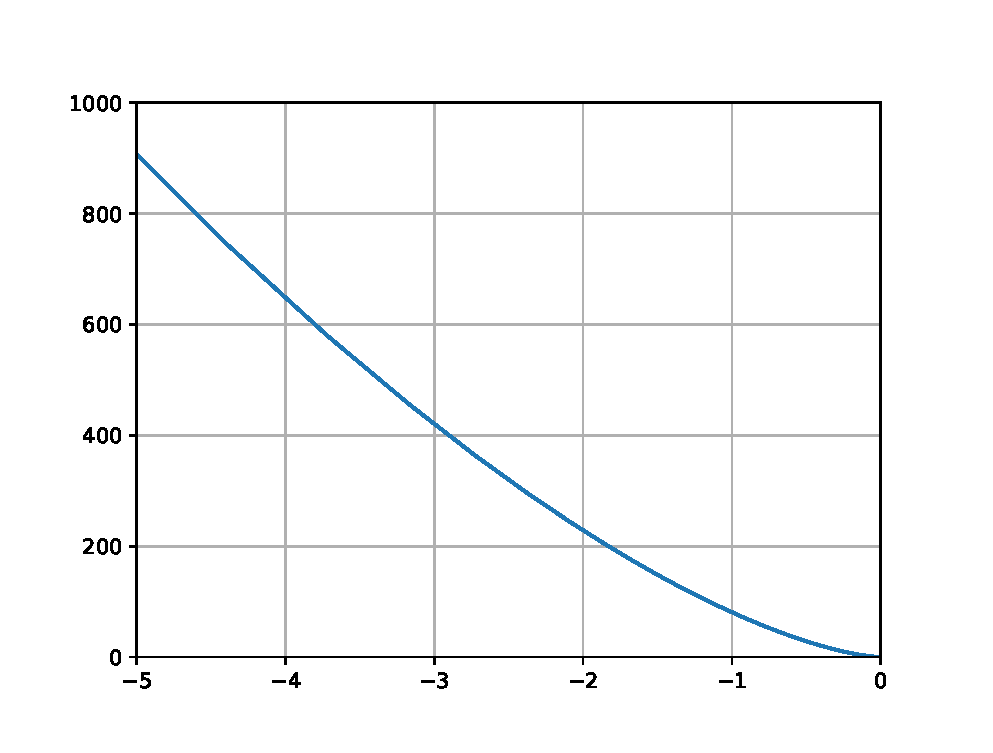
\includegraphics[width=\columnwidth]{./figs/ee18btech11029.eps}
  \caption{}
  \label{fig:ee18btech11029}
\end{figure}

\begin{itemize}
    \item The polar plots use open loop transfer function to determine the stability and hence reference point is shifted to \brak{-1,0}
    \item If \brak{–1,0} is left of the polar plot or \brak{–1,0} is not enclosed, then it is stable
    \item If \brak{–1,0} is on right side of the polar plot or \brak{–1,0} is enclosed by polar plot then it is unstable. 
    \item If \brak{–1,0} is on the polar plot then it is marginally stable
    
\end{itemize}

In Fig.   \ref{fig:ee18btech11029},  \brak{-1,0} is on the polar plot so the system is marginally stable.
   
\end{enumerate}
